\documentclass[]{sig-alternate}
 \usepackage{booktabs}
\usepackage[caption=false]{subfig}
 \usepackage[colorinlistoftodos,backgroundcolor=yellow]{todonotes} %disable
 \usepackage{color}

\newcommand{\XXX}[1]{\textcolor{red}{{\it \textbf{[XXX: #1]}}}}
\hyphenation{Max-DB data-base}

\usepackage{comment}
\newtheorem{mydef}{definition}
\usepackage{graphicx}
\newcommand{\slbl}[1]{\textbf{\textsf{#1}}}
\usepackage{multirow}%,multicolumn}
\usepackage{slashbox}
\usepackage{wrapfig}
\usepackage{booktabs, colortbl}
\usepackage{amsmath}
\usepackage{url}
\usepackage[pdfstartview=FitH,bookmarksopenlevel=3,bookmarks=true]{hyperref} %pdfpagescrop={92 112 523 778},

% % share affiliation and use less space
% \def\sharedaffiliation{%
% \end{tabular}
% \begin{tabular}{c}}
% %

\begin{document}

\conferenceinfo{MSR}{'11 Waikiki, Hawaii, USA}

\numberofauthors{4}

\author{
\alignauthor 
Abram Hindle\\
   \affaddr{Dept. of Computer Science}\\
   \affaddr{University of California, Davis} \\
   \affaddr{Davis, CA, USA}\\
   \email{\large abram@softwareprocess.es}
\alignauthor  Neil A. Ernst\\
   \affaddr{Dept. of Computer Science}\\
   \affaddr{University of Toronto}\\
   \affaddr{Toronto, Ontario, CANADA}\\
   \email{\large nernst@cs.toronto.edu}
\and
\alignauthor Michael W. Godfrey\\
   \affaddr{David Cheriton School of Computer Science}\\
   \affaddr{University of Waterloo}\\
   \affaddr{Waterloo, Ontario, CANADA}\\
   \email{\large migod@uwaterloo.ca}
\alignauthor John Mylopoulos \\
   \affaddr{Dept. Information Eng. and Computer Science}\\
   \affaddr{University of Trento}\\
   \affaddr{Trento, ITALY}\\
   \email{\large jm@disi.unitn.it}
}

%\title{What's in a name? Automated topic naming of software maintenance activities}
\title{Automated topic naming to support cross-project analysis of software maintenance activities}
\maketitle
%\thispagestyle{empty}

\begin{abstract}
% %\todo[inline]{Topics and LDA sooner, Topics/concept location is a known
Researchers have employed a variety of techniques to extract underlying
topics that relate to software development artifacts.  Typically, these
techniques use unsupervised machine-learning algorithms to suggest
candidate word-lists.  However, word-lists are
difficult to 
interpret in the absence of meaningful summary labels.  Current topic modeling 
techniques assume manual labelling and do not use domain-specific knowledge
to improve, contextualize, or describe results for the developers.  
We propose a solution: \emph{automated labelled topic extraction}.
  Topics are extracted 
using  Latent Dirichlet Allocation (LDA) from commit-log comments recovered
from source control systems such as CVS and BitKeeper.  
These topics are given labels from a generalizable
cross-project taxonomy, consisting of non-functional
requirements. Our approach was evaluated with experiments and case studies
on two large-scale RDBMS projects: MySQL and MaxDB.  The case studies
show that labelled topic extraction can produce appropriate,
context-sensitive labels relevant to these projects, which provides fresh
insight into their evolving software development activities.
\end{abstract}

\category{D.2.9}{Software Engineering}{Management}[Lifecycle]
\category{D.2.1}{Software Engineering}{Requirements/Specifications}[Tools]

%\terms{Theory}

\keywords{Topic analysis, LDA, non-functional requirements}

\newcommand{\shrink}{}
\section{Introduction}

%\todo[inline]{Strength story: Neil says
  % And ultimately, I think the story needs more strengthening. Maybe we
  % need a scenario: you work at Bank X. You are curious about how much
  % recent activity has been done on software maintainability
  % vs. security. Our technique will allow you to compare different IT
  % projects using the same keywords, and ultimately, to generate lists
  % showing relative frequencies.}

% \todo[inline]{mention project dashboards}

% % \todo[inline]{Usefulness needs to be immediate and apparent}

% \todo[inline]{ It needs to be clear there is value in labelling.
 %  We need to make it clear that other researchers weren't labelling them
 % automatically and presented them as labelled and thus it is obvious from
 %  their presentation that labels matters + need a reading argument. The
 % 2nd reviewer picked on this a bit but still didn't get it. I thought
 % some of this had been clear.}

%\todo[inline]{Topic should be defined clearly (italics and hilighted)}

% \todo[inline]{Move previous work up}

%One challenge for software maintenance is to identify the reasons
%behind software development activities. 
%Identifying these reasons provides insight into \emph{why} certain
%changes were made. 
%migod
A key problem for practising software maintainers is gaining an understanding of \emph{why} a system has evolved the way it has. Looking back on streams of artifacts scattered across different repositories, inferring what activities were performed, when, and for what reasons, is hard to do without expert advice from the developers involved. In this work we seek to provide automated help in labelling development topics that have been extracted from commit logs.

Topic modeling is a machine learning technique which creates
multinomial distributions over words from a text corpus. 
The technique infers the hidden structure of a corpus using posterior
inference: the probability of the hidden structure given the data. 
Topic models are useful in software maintenance because they summarize
the key concepts in a corpus, such as source code, commit comments, or
mailing-list messages, by identifying statistically co-occurring words. 
Among other uses, it can quickly give developers an overview of where significant
activity has occurred, and gives managers or maintainers a sense of
project history. 
For example, a topic extracted from a set of commit logs might consist of the following terms: \emph{ ``listener change remove add fire''}. 
%A major challenge for topic modeling is to accurately identify the
%summary label for a topic; in the previous case, perhaps
%\emph{``event-handling''} would be appropriate. 
%Current approaches are manual: they rely on human expertise to
%recognize the appropriate label. 
%Furthermore, to date the results of topic modeling are project
%specific, and not generalizable. 
%This paper presents an approach, \emph{labelled topic extraction}, which addresses these two problems.

%migod
While machine learning techniques can automatically identify clumps of commonly recurring terms, devising an appropriate summary label for each clump/topic is harder.  For example, the word list above might reasonably be labelled as \emph{"event handling"} by a human who understands the domain well, despite the fact that label does not appear in the word list itself.  Current approaches to topic labelling rely on manual intervention by human experts, and also are limited to project-specific topic labels.  In this paper, we introduce \emph{labelled topic extraction}, an approach to topic labelling that is both automatic and creates labels that are project independent.

% Changes to software systems, revisions, do not occur without
% reason. 
% The reason or purpose is often related to requirements 
% Often one revision might have multiple purposes ranging from
% maintenance issues, quality issues, requirements, features or a
% response to a bug report.
% These purposes often are exhibited as latent topics that relate to
% many development artifacts such as:
%  version control revisions, bug reports, and mailing-list discussions.

%In our previous work we dealt with topic trends, which are topics that recur over time~\cite{Hindle09ICSM}. 
%We observed that topic trends were often non-functional requirements (NFRs). 
%NFRs have the property of being cross-domain and widely applicable. 
%In this sense, they are useful abstractions for developer conversations about different software projects.

% harp on data mining more
%In general, the mining of software artifacts tends to be very project specific, yet NFRs are not. 
% I was told if you're going to use a paren, you don't need to say it.
%There is a series of standards on NFRs, such as ISO9126~\cite{iso9126}, specifically intended to apply to projects of varying types.
%These standards indicate our approach is possible. %, if perhaps not universally accepted).
% NFRs are prevalent in almost all software systems.
% In this paper we will show that NFR related topics occur quite frequently.
%XXXXXX this sentence is confusing
%This informs our method of generalizing the data mining of these software artifacts to leverage the global domain knowledge of software engineering, specifically NFRs. 
%In particular, we use software quality models to generalize topics across projects. 
%This allows us to mine software systems with the intention of comparing their NFR-related development topics.
% in order to achieve generalizable, cross project data mining results.

%%%% THIS PARAGRAPH ARGUES ABOUT THE CONCRETE APPLICATION OF 
%%%% TOPIC MODELLING AND LABELLED TOPIC EXTRACTION
%%%% IT NEEDS TO BE TIGHTER BUT IT ALSO NEEDS TO BE HERE

% AH: Topics take a long to read
% AH: Project Dashboards, summarization, software process recovery

%migod
In general, the fruits of mining software artifacts are often project specific and hard to generalize.  However, in our previous work we investigated \emph{topic trends} --- that is, topics that recur over time --- we observed that topic trends often corresponded to non-functional requirements (NFRs) \cite{Hindle09ICSM}.  This is encouraging, as NFRs have the property of being cross-domain and widely applicable. In this sense, they are useful abstractions for developer conversations about different software projects.  Furthermore, there is a series of standards on NFRs, such as ISO9126 \cite{iso9126}, that are specifically intended to apply to projects of varying types; this suggests that our goal of trying to extract NFR-related development topics, such as those related to software quality models, holds promise.

Concrete applications of topics and \emph{labelled topic extraction}
range from project dashboards to annotating software artifacts such as revisions and bug reports with
NFR-related tags.
Project dashboard are typically employed by managers and are used to
provide quick summaries of the effort put into a software project. In this case, 
labelled topic extraction would allow managers to track effort
related to topics, such as usability or other NFRs.
These techniques also allow for the annotation of commit comments
 and other software artifacts with NFRs. 
This would enable querying of bug reports and artifacts by relevant NFRs. 
For instance one could look
for \emph{usability}-relevant revisions and bug reports.


%% RESEARCH DIDNT DO THIS AND WE ARE TOTALLY AWESOME AND WE DID
% it is ok to repeat this here because it is clear and bullet pointed and the reviewers wont have any bloody excuse to not see it
In this paper, we describe \emph{labelled topic extraction}. It addresses two gaps in the topic mining literature:
\begin{enumerate}
  \item Topic mining of software has been limited to one project at a time. 
This is because traditional topic mining techniques are specific to a particular data-set. 
\textit{Labelled topic extraction} allows for comparisons \textit{between} projects. 
  \item Topic modeling creates word lists that require interpretation by the user to assign meaning. 
Like (1), this means
that it is difficult to discuss results independent of the project context. 
Our technique automatically, or with some initial training, assigns labels across projects.
\end{enumerate}

This paper makes the following contributions: 
\begin{itemize}
\item introduces the concept of labelled topic extraction, using a non-functional requirements (NFR) taxonomy for our labels. 
\item evaluates an unsupervised method of automated topic labelling (word-lists);
%\item Our unsupervised method can be applied to projects without training;
\item evaluates a supervised method of automatically labelling topics with a single NFR (machine learning);
\item evaluates a supervised method of labelling topics with multiple NFRs (multi-label machine learning);
\item provides a method of cross-project analysis via topic labelling; and
\item applies these techniques to visualize NFRs over time, and to analyze maintenance activities.
\end{itemize}

%We first introduces labelled topic extraction, and then uses that technique to analyze development activity in two large-scale examples.
We begin by discussing related work in Section \ref{sec:related}.
Next, we describe how we generated our data (Section \ref{sec:wordlist}). For unsupervised classification (Section \ref{sec:unsuplabelling}), we begin by creating word-lists to signify when a topic matches an NFR label. We then apply our classifier and analyze the results. %and how we created the word-lists used in unsupervised classification. 
%We show that labels with their topics can be learned and used to classify other data-sets, either without training 
%Our goal is to label a given topic with either an NFR from our taxonomy,
 %Section \ref{sec:unsuplabelling} presents our technique for using word-lists to do unsupervised classification, and describes the results.
In Section \ref{sec:suplabelling}, we manually annotate the topics, and use those annotations as training data for supervised classification.  
%We then present visualizations of named topics and their trends over time to aid communication and analysis. 
To demonstrate an application of labelled topic extraction, we use an exploratory case study of two open source database systems to show how named topics can be compared between projects  (Section \ref{sec:analysis}). 
The paper concludes with a discussion of limitations (Section \ref{sec:limit}), and future work.

%\todo[inline]{Topics are poorly defined by this point and since we're building on research which didn't DO this, we should mention that research. Previous work probably should go here.}

%\todo[inline]{We still haven't shown that topics are useful -- a reviewer comment}


\section{Previous Work}
\label{sec:related}

The idea of extracting higher-level \emph{concerns}, also known as \emph{concepts}, \emph{aspects} or \emph{requirements}, has been approached from documentation-based and repository-based perspectives.

Cleland-Huang and her colleagues published work on mining requirements documents for non-functional requirements (NFR) (quality requirements)~\cite{Cleland-Huang2006}. 
Their approach was similar to ours, as they mined keywords from NFR catalogues.
%One approach they tried was similar to this one, with keywords mined from NFR catalogues found in their previous work~\cite{chung99}. 
They managed a recall of 80\% with precision of 57\% for the Security NFR, but could not find a reliable source of keywords for other NFRs. 
Instead, they developed a supervised classifier by using human experts to identify an NFR training set. 
Our work differed because we had a more comprehensive set of terms based on the taxonomy we chose.
We make cross-project comparisons, while they focused on a single project.
%The objective of Cleland-Huang's study was to identify new NFRs for system development, yet our objective was to recover those latent NFRs from commit-log messages of the project. 
Another difference was that our data was far less structured than the requirements documents used in their study.
%There are several reasons we did not follow this route. 
%One, we believe we have a more comprehensive set of terms due to the taxonomy we chose. 
%Secondly, we wanted to compare across projects. 
%Their technique was not compared across different projects and the applicability of the training set to different corpora is unclear. 
%A common taxonomy allows us to make cross-project comparison. 
%Although subject to the assumption that all projects conceive of these terms in the same way.
%Thirdly, while the objective of Cleland-Huang's study was to identify new NFRs (for system development) our study assumes these NFRs are latent in the commit-log messages of the project. 

Similarly, Mockus and Votta~\cite{Mockus00} studied a large-scale industrial change-tracking system. 
They also leveraged WordNet, but only for word roots as they felt the synonyms would be non-specific and cause errors, problems we also encountered. 
Mockus et al. had access to system developers, with whom they could validate their labels. 
Since we try to bridge different organizations, instead of a single project, these kind of interviews are infeasible (particularly in the distributed world of open-source software).

The other approach is to extract concerns from software repositories.
Marcus et al.~\cite{marcus04wcre} describe their use of Latent Semantic Indexing (LSI) to identify commonly occurring concerns for software maintenance. The concerns are given by the user, and LSI used to retrieve them from a corpus. Topic modelling generates topics that are independent of a user query, and relate only to word frequencies in the corpus.
%Some results were interesting, but their precision was quite low. 
With ConcernLines, \cite{treude09cl} shows tag occurrence using colour intensity. 
They mined 
developer created tags 
%change request tags (such as `milestone 3') and used these 
in order to analyze the evolution of a single product.
% make evolutionary analyses of a single product. 
The presence of a well-maintained set of tags is obviously essential to the success of this technique.

%XXXXXXXXXXXX OPTIONAL
% Not sure we need this
%Mens et al.~\cite{mens08icsm} conducted an empirical study of Eclipse, a popular Java IDE, to verify the claims of Lehman~\cite{lehman97sms}.
% They concerned themselves with source code only, and found Law Seven, ``Declining Quality'', to be too difficult to assess: ``[we lacked an] appropriate measurement of the evolving quality of the system as perceived by the users \cite[p. 388]{mens08icsm}''. 
%This paper examines the notions of quality in terms of a consistent ontology, as Menset al. call for in their conclusions.

% in our previous work~\cite{Hindle09ICSM}, as well as -- CITED a little too often (vanity cites!)
In Baldi et al.~\cite{Baldi2008}, topics are named manually: human experts read the highest-frequency members of a topic and assign a label accordingly. 
As discussed earlier, given the topic \emph{``listener change remove add fire''}, Baldi et al. would assign the label \emph{event-handling}. 
The labels are reasonable enough, but still require an expert in the field to determine them. 
Furthermore, these labels are project-specific, because they are generated from the data of that project. E.g., we might have a label called `Oracle' in the MySQL case, since Oracle owns MySQL. 
We do this differently.
%This paper does this differently. 
First of all, we automated the process of naming the topics. Secondly, we labelled topics with project-independent terms, in order to permit cross-project comparison.

Mei et al.~\cite{Mei2007} use context information to automatically name topics. 
They describe probabilistic labelling, using the frequency distribution of words in a topic to create a meaningful phrase. 
They do not use external domain-specific information as we do.

Finally, in \cite{ernst10refsq}, we describe our earlier project, similar to this, to identify change in quality requirements in GNOME software projects; our approach is solely text-matching, however, and does not leverage machine learning strategies.

%Massey~\cite{massey02icse} and Scacchi~\cite{scacchi02,scacchi05b} looked at the topic of requirements in open-source software. 
% this reduces the line length and drops a ref even though we still have a scacchi kickin around
%Massey~\cite{massey02icse} and Scacchi~\cite{scacchi05b} looked at the topic of requirements in open-source software. 
%Their work discusses the source of the requirements and how they are used in the development process. German~\cite{german03gnome} looked at GNOME specifically, and listed several sources for requirements: leader interest, mimicry, brainstorming, and prototypes. 
%None of this work  addressed quality requirements in OSS, nor did it examine requirements trends.

% XXX vanity or space.. 
%XXXXXXXXXXXX OPTIONAL
% NE 0113 this seems too early to mention 'result'.
% Hindle et al. \cite{Hindle2007} examined release patterns in OSS. They showed that there is a difference between projects regarding maintenance techniques. This supports our result that software qualities are not discussed with the same frequency across projects.


\section{Study design and execution}
Figure \ref{fig:process} gives an outline of methodology.
We began by gathering source data and creating topic models. For unsupervised labelling, we generated three sets of word-lists as signifiers for NFRs.
%e created labels using a well-known NFR taxonomy. 
In supervised learning, we trained our data with manual annotations in order to match topics with NFRs. Finally, these topics were used to analyze the role of NFRs in software maintenance.

\begin{figure}
  \centering
 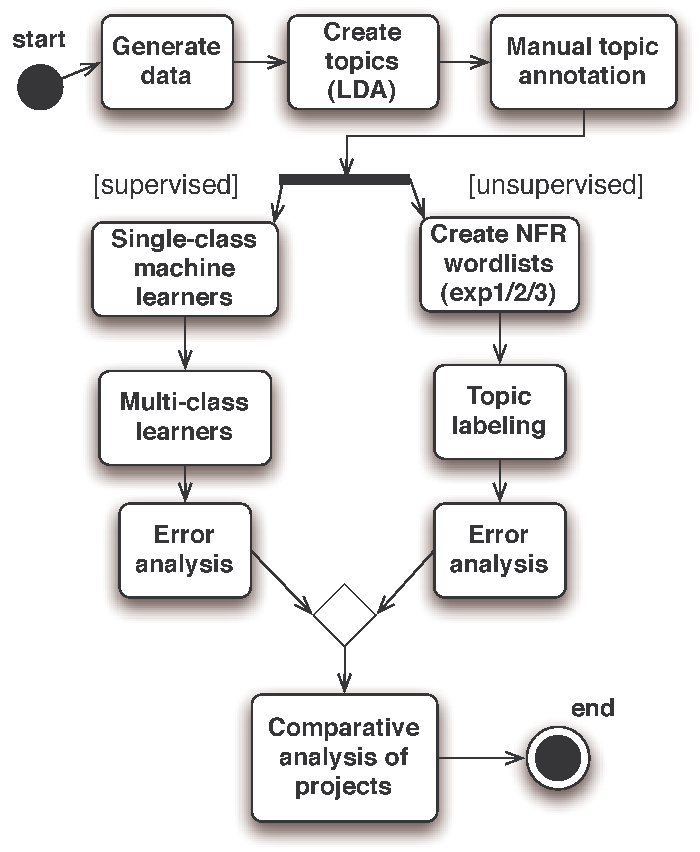
\includegraphics[width=.45\textwidth]{figures/process-model}
 \caption{Research methodology process view.}
  \label{fig:process}
\end{figure}

\subsection{Generating the data}
\label{sec:wordlist}

To evaluate our approach, we sought candidate systems that were mature projects and had openly accessible source control repositories. 
We selected systems from the same application domain, to control for differences in functional, rather than non-functional, requirements. 
We selected MySQL 3.23 and MaxDB 7.500 as they were open-source, partially-commercial database systems. 
MaxDB started in the late 1970s as a research project, and was later acquired by SAP. 
As of version 7.500, released April 2007, the project has over $940,000$ lines of C source code\footnote{generated using David A. Wheeler's \emph{SLOCCount}, dwheeler.com/sloccount.}. 
The MySQL project started in 1994 and MySQL 3.23 was released in early 2001. 
MySQL contains $320,000$ lines of C and C++ source code.  
%Choosing an older version of these projects allowed us to focus on projects which have moved further into the maintenance phase of the software life-cycle.
For our study, we explicitly chose older versions of mature projects from a stable problem domain to increase the likelihood that we would encounter primarily maintenance activities in our studies.


For each project, we used source control commit comments, the messages
that programmers write when they commit revisions to a source control
repository. 
Commit comments are often studied by researchers, as they are the most readily accessible source of project interactions, and developers are often required to create them by the repository mechanism (e.g., Git).  Additionally, relying only on commit comments makes our approach more generalizable, as we do not assume the presence of other artifact corpora.
%This is the most readily accessible source of project interactions for outside researchers, since developers often or always (e.g., Git) write such message. Our approach is more generalizable if it does not assume the presence of other corpora. %bug trackers and email-list archives were not available for both projects. 
An example of a typical commit message, from MySQL, is: \textit{``history annotate diffs bug fixed (if mysql\-\_real\-\_connect() failed there were two pointers to malloc'ed strings, with memory corruption on free(), of course)''}. 
We extracted these messages and indexed them by creation time. 
We summarized each message as a word distribution but removed stop-words such as ``\emph{the}'' and ``\emph{at}''. 
%Stemming was performed in the later stages of our analysis. % WAS IT?

For the commit message data-sets of each project, we created an XML file that separated commits into 30 day periods. 
%This size of period, 30 days, is smaller than the time between minor
%releases but large enough for there to be sufficient commits to
%analyze
We chose a period size of 30 days as it is smaller than the time between minor releases but large enough for there to be sufficient commits to analyze~\cite{Hindle09ICSM}. 
For each 30 day period of each project, we input the messages of that period into Latent Dirichlet Allocation (LDA), a topic analysis algorithm~\cite{Blei2003}, and recorded the topics the algorithm extracted.
%For each project and for each period of messages a project, we input these messages 
%we created `topics' using Latent Dirichlet Allocation, a topic identification algorithm. 

A topic analysis tool such as LDA will try to find $N$ independent
word distributions within the word distributions of all input messages. 
Linear combinations of these $N$ word distributions are meant to represent and recreate the word distributions of any of the original messages. 
These $N$ word distributions effectively form topics: cross-cutting collections of words relevant to one or more of our commit messages. 
LDA extracts topics in an unsupervised manner; the algorithm relies
solely on the source data and word distributions of messages, with no human intervention.

In topic analysis a single document, such as a commit message, can be related to multiple topics. 
Representing documents as a mixture of topics maps well to source code repository commits, which often have more than one purpose~\cite{Hindle09ICSM}.  
For this paper, a topic represents a word distribution generated from a group of commit log comments which are related by their content.  
%In this paper a topic is a set of tokens extracted from commit messages found within a project's source control system (SCS).

We applied Blei's LDA implementation~\cite{Blei2003} against the word distributions of these commits, and generated lists of topics per period. 
We set the number of topics to generate to $20$, because past experimentation showed that fewer topics might aggregate multiple unique topics while any more topics seemed to dilute the results and create indistinct topics~\cite{Hindle09ICSM}. 
% Furthermore, more than $20$ topics quickly became infeasible for inspection.

\subsubsection{The high-level labels}

%\noindent \textbf{The high-level labels} --- 

To facilitate cross-project comparison, we used a taxonomy of NFRs. This taxonomy is based on the ISO quality model, ISO9126~\cite{iso9126}. 
ISO9126 describes six high-level NFRs: maintainability, functionality,
portability, efficiency, usability, and reliability~\footnote{While there may be lingering debate in some circles about these terms, an ISO standard seems like a reasonable starting point for our work.}
%There is some debate about the terms in this model. 
%However, ISO9126 is ``an international standard and thus provides an internationally accepted terminology for software quality \cite[p. 58]{Boegh2008},'' that is sufficient for the purposes of this research.  
We claim that these NFRs are maintenance concerns (to varying degrees) in all software projects, and are therefore well-suited to comparison between projects.

%\noindent \textbf{Creating a validation corpus} --- 
\subsubsection{Creating a validation corpus}
To evaluate both unsupervised and supervised classification, we
created a validation set of manually labelled topics. For MySQL 3.23
and MaxDB 7.500, we annotated each extracted topic in each period with
the six NFR labels listed above.
We looked at each period's topics, and assessed what the data --- consisting of the frequency-weighted word lists and messages --- suggested was the topic for that period. 
We were able to pinpoint the appropriate label using auxiliary information as well, such as the actual revisions and files that were related to the topic being annotated.
For example, for the MaxDB topic consisting of a message ``exit() only used in non NPTL LINUX Versions'', we tagged that topic \emph{portability}. 
%\todo[inline]{this confused people. Is it truly unsupervised? Yes, but it needs to be clearer.}
%We compared against this data-set, but we also used the data-set for our supervised machine learning based topic classification. 
% A topic may have more than one matching keyword. % ok what?
%\todo[inline]{inter-rater reliability }
% \todo[inline]{There should be a section here which is about manual annotation. It is really important and it is required by both analyses. Plus we can tell them how.}

%\todo[inline]{NEIL: this section should be updated to explain F-measure}
We validate classification performance using the Receiver Operating
Characteristic area-under-curve value~\cite{Fawcett2006861},
abbreviated \emph{ROC}, and the F-measure, which is the harmonic mean of precision and recall, i.e., $2 * (P * R) / (P + R)$. 

%\todo[inline]{NEIL: abram, i got rid of the letter-grade thing because I'm worried people latch on to the idea we are C- students. I feel anything better than random is our criteria here}
ROC values provide a score %, similar to school letter-grades (A is 0.9, C is 0.6),
 reflecting how well a particular learner performed for the given data. 
ROC maps to the more familiar concepts of precision/sensitivity and recall/specificity: it plots the true positive rate (sensitivity) versus the false positive rate (1 - specificity). 
A perfect learner has a ROC value of 1.0, reflecting perfect recall and precision. 
A ROC result of 0.5 would be equivalent to a random learner (that is, issuing as many false positives as true positives). 
The %area under the -- NE confusing to have area again ... and not importantana
ROC of a classifier is equivalent to the probability that the classifier will rank a randomly chosen positive instance higher than a randomly chosen negative instance.

We consider our labelling classifiers acceptable if they outperform a random classifier (0.5). 

\subsection{Unsupervised labelling}
\label{sec:unsuplabelling}

In this section we describe how to label topics based on dictionaries
mined from sources external to the projects themselves.

%\subsection{Generating word lists}
%\label{sec:genwordlist}
% %\todo[inline]{Make it clear where the data comes from! Neil says: Also, I
%   didn't get the impression they understood that we weren't generating
%   labels from the data, but rather from independent taxonomies. Of
%   course if you use labels from the data it isn't comparable. But the
%   point of ISO 9126 etc. was to avoid exactly this problem.}

% \todo[inline]{Need to hammer it in that the word bags are not project specific and
%  are inherited so it isn't a supervised method}


%Topics are word distributions, lists of words ranked by frequency, that are burdensome to interpret and hard to distinguish and understand. 
%While the topics themselves are generated automatically, how to interpret these topics is less clear.
%For example,

\subsubsection{Generating word lists}

%\noindent\textbf{Generating word lists} --- 

In order to automatically label each topic with 
one of the six high-level NFRs,
%an NFR from ISO9126, 
we associate each NFR with a list
of keywords (`word-lists', in our parlance). These word-lists were determined a priori and were not extracted from the projects themselves.
We intersected the words of the topics and the words of our word-lists.
We ``labeled'' a topic if any of its words matched any of the word-list's words.
A topic could match more than one NFR.
We used several different sets of word-lists for comparison, which we
refer to as \textsf{exp1}, \textsf{exp2}, and \textsf{exp3} in the text which follows. 

Our first word-list set, \textsf{exp1}, was generated using the ontology described in Kayed et al.~\cite{5072519} .
That paper constructs an ontology for software quality measurement using eighty source documents, including research papers and international standards. 
The labels we used:
\begin{quotation}
\small \noindent \textsf{
integrity, security,
interoperability, testability, maintainability, traceability,
accuracy, modifiability, understandability, availability, modularity,
usability, correctness, performance, verifiability, efficiency,
portability, flexibility, reliability.
}
\end{quotation}

Our second word-list, \textsf{exp2}, uses the ISO9126 taxonomy described above (Section \ref{sec:wordlist}) to seed the word-lists.
%We use these qualities later on as classes in supervised labelling. NE confusing the issue here, I think.
The terms from ISO9126 may not capture all words occurring in the topics that are nonetheless associated with one of the NFRs. 
For example, the term ``redundancy'' is one 
we considered to be
relevant to discussion of reliability, but is not in the standard. 
We therefore took the NFRs from the ISO9126 and added to them.

%\todo[inline]{* clarify the mailinglist stuff we did}
%\todo[inline]{This part doesn't make a lot of sense}
To construct these expanded word-lists, we used WordNet~\cite{Fellbaum1998}, an English-language ``lexical database'' that contains semantic relations between words, including common related forms (similar to word stemming), meronymy and synonymy. 
We then added Boehm's software quality model \cite{Boehm+:1976:ICSE}, and classified his eleven `ilities' into their respective ISO9126 NFRs. 
We did the same for the quality model produced by McCall et al. \cite{mccall1977}. 
We then did a simple random analysis of mailing list messages from an open source project, KDE. If we judged a given message to contain terms that were related to one of the NFRs in ISO9126, we added it to our word-list. This allowed us to expand our word-lists with more software-specific terms.
%Finally, we randomly analyzed two mailing lists from another software project to expand our set with domain-specific terms. 
% Less info is probably better here...
%For example, we add the term ``performance'' to the synonyms for \emph{efficiency}, since this term occurs in most mail messages that discuss efficiency.  Table \ref{tbl:wnsig} shows the labels (NFRs) and word-lists we used for matching.

For the third set of word-lists, \textsf{exp3}, we extended the word-lists from \textsf{exp2} using unfiltered WordNet similarity matches. 
Similarity in WordNet means siblings in a hypernym tree. 
We do not include these words here for space considerations (but see the Appendix for our data repository). 
It is not clear the words associated with our labels in \textsf{exp3} are specific enough. For example, the label \emph{maintainability} is associated with words \emph{ease} and \emph{ownership}. In general, as we proceed from word-list in \textsf{exp1} to that in \textsf{exp3}, our lists get more generic.

\begin{table*}
	\centering
\begin{tabular}{c|p{11cm}}
\toprule
\textbf{Label} & \textbf{Related terms} \\
\midrule
\emph{Maintainability} &
testability changeability analyzability stability maintain maintainable modularity modifiability understandability interdependent dependency encapsulation decentralized modular\\ \hline
\emph{Functionality} &
security compliance accuracy interoperability suitability functional practicality functionality compliant exploit certificate secured ``buffer overflow'' policy malicious trustworthy vulnerable vulnerability accurate secure vulnerability correctness accuracy\\ \hline
\emph{Portability} &
conformance adaptability replaceability installability portable movableness movability portability specification migration standardized l10n localization i18n internationalization documentation interoperability transferability\\ \hline
\emph{Efficiency} &
``resource behaviour'' ``time behaviour'' efficient efficiency performance profiled optimize sluggish factor penalty slower faster slow fast optimization\\ \hline
\emph{Usability} &
operability understandability learnability useable usable serviceable usefulness utility useableness usableness serviceableness serviceability usability gui accessibility menu configure convention standard feature focus ui mouse icons ugly dialog guidelines click default human convention friendly user screen interface flexibility\\ \hline
\emph{Reliability} &
``fault tolerance'' recoverability maturity reliable dependable responsibleness responsibility reliableness reliability dependableness dependability resilience integrity stability stable crash bug fails redundancy error failure\\ 
\bottomrule
\end{tabular}
	\caption{NFRs and associated signifiers -- \textsf{exp2}}
	\label{tbl:wnsig}

\end{table*}

\subsubsection{Automatic Labelled Topic Extraction}

%\todo[inline]{NEIL: this could be a subsubsection}
%\todo[inline]{* the hierarchy of tags was not clear}
%\noindent \textbf{Generating labels automatically} --- 

Using our three word-lists (\textsf{exp1}, \textsf{exp2}, \textsf{exp3}), we labeled our topics with an NFR where there was a match between a word in the list and the same word somewhere in the distribution of words that constitute the topic.
A \emph{named topic} is a topic with a matching NFR label. Unnamed topics occur where this no such match, which may indicate either a lack of precision, or simply that this topic is not associated with non-functional requirements.
All experiments were run on MaxDB 7.500 and MySQL 3.23 data. LDA
extracted 20 topics per period for each.
% Is this good enough
This labelling is unsupervised because the corpus is not derived from 
the project being labelled, and we did not label the project's topics
ourselves for a training set. The motivation behind this technique is that
because most software often addresses similar issues, we can use the
domain knowledge of software to label relevant topics.
%\todo[inline]{Neil does this explain the unsupervised aspect well enough?} 

Table \ref{tbl:wordlist} shows how many topics were labelled for MaxDB
and MySQL.


%\todo[inline,color=green]{this table should have mysql}
\begin{table}

% % This data came from running  
% %   python check_validity.py
% %  in src/validate
% % and then running
% % tail -n 5 *maxdb*yes_no*
% % tail -n 5 *mysql*yes_no*
% ok the new way is to run lda_relator
% src/validate/lda_relator_counts.sh
	\centering
\begin{tabular}{l|c|c|c|c}
\toprule
\textbf{Project} & \textbf{Measure} & \textsf{exp1} & \textsf{exp2} & \textsf{exp3} \\
\midrule
% NOTE THESE WERE THE OLD VALUES
% WHY DID THEY CHANGE???
% DUNNO
%Named topics   & 281 & 125 & 328  \\
%Unnamed topics & 139 & 295 & 92   \\

% these were check_validate
% MaxDB 7.500 & Named Topics   & 305 & 183 & 330 \\
% MaxDB 7.500 & Unnamed Topics & 84  & 206 & 59   \\
% MaxDB 7.500 & Total  Topics  & 389 & 389 & 389 \\
% MySQL 3.23  & Named Topics   & 341 & 202 & 469 \\
% MySQL 3.23  & Unnamed Topics & 245 & 384 & 117 \\
% MySQL 3.23  & Total  Topics  & 586 & 586 & 586 \\

% these are lda relator

MaxDB 7.500 & Named Topics   & 281 & 125 & 328 \\ % these numbers are
                                % slightly different solely because
                                % we're counting empty topics
                                % maxdb has 80 empty topics
 & Unnamed Topics & 219  & 375 &  172  \\
 & Total  Topics  & 500 & 500 & 500 \\
\midrule
MySQL 3.23  & Named Topics   & 524 & 273 & 773 \\
  & Unnamed Topics & 476 & 727 & 227 \\
  & Total  Topics  & 1000 & 1000 & 1000 \\


\bottomrule
\end{tabular}
	\caption{Automatic topic labelling for MaxDB and MySQL}% \todo[inline]{this stupid table is before table 1}}
	\label{tbl:wordlist}

\end{table}

For \textsf{exp1}, our best performing 
labels --- that is, those with the most topics --- were
%labels, those with the most topics, 
\emph{correctness} (182 topics) and \emph{testability} (121). 
We did not get good results for \emph{usability} or \emph{accuracy}, which were associated with fewer than ten topics. 
We also looked for correlation between our labels: Excluding double matches (self-correlation), our highest co-occurring terms were \emph{verifiability} with \emph{traceability}, and \emph{testability} with \emph{correctness} (76 and 62 matches, respectively).
% See the following sections for our error analysis. 

For \textsf{exp2}, there are more unnamed topics than \textsf{exp1}. 
Only \emph{reliability} produces a lot of matches, mostly with the word ``error''. 
Co-occurrence results were poor. This suggests our word lists were overly restrictive.

For \textsf{exp3}, we generally labelled more topics. 
As we mentioned, the word-lists are broad, so there are likely to be false-positives (discussed below). 
We found a high of 265 topics for \emph{usability}, with a low of 44 topics for \emph{maintainability}. 
Common co-occurrences were \emph{reliability} with \emph{usability}, \emph{efficiency} with \emph{reliability}, and \emph{efficiency} with \emph{usability} (200, 190, and 150 topics in common, respectively). 


%\todo[inline]{Should we use F-1 as well to satisfy everyone?}

\subsubsection{Analysis of the unsupervised labelling} %--- %Based
                                %on the labels, and our manual topic
                                %labelling, 
%\noindent \textbf{Analysis of the unsupervised labelling} --- %Based on the labels, and our manual topic labelling, 
%we compared the results of the unsupervised word matching approach. 
For each quality we assessed whether unsupervised labels matched the manual annotations. %To be clear, the manual annotations were not used to train the labeling process.
As described in \ref{sec:wordlist} we used both ROC and F-1 measures to evaluate the performance of the classification.
Figure \ref{fig:maxdb-unsup-results} shows our ROC results for MaxDB and MySQL. We describe F-1 results in the text below.


%\todo[inline]{since ROC is new-sounding, I wonder if a more lengthy explanation would be merited. An obvious question is why not precision/recall? -- ROC is hot right now and it combines both}
% Rebuttal: ROC is not new and it is what the machine learning community, search based software engineering and now the MSR community are using +  it has natural meaningful quality mappings.
% \begin{figure}[t]
% \centering
% \subfloat[ROC]{
%  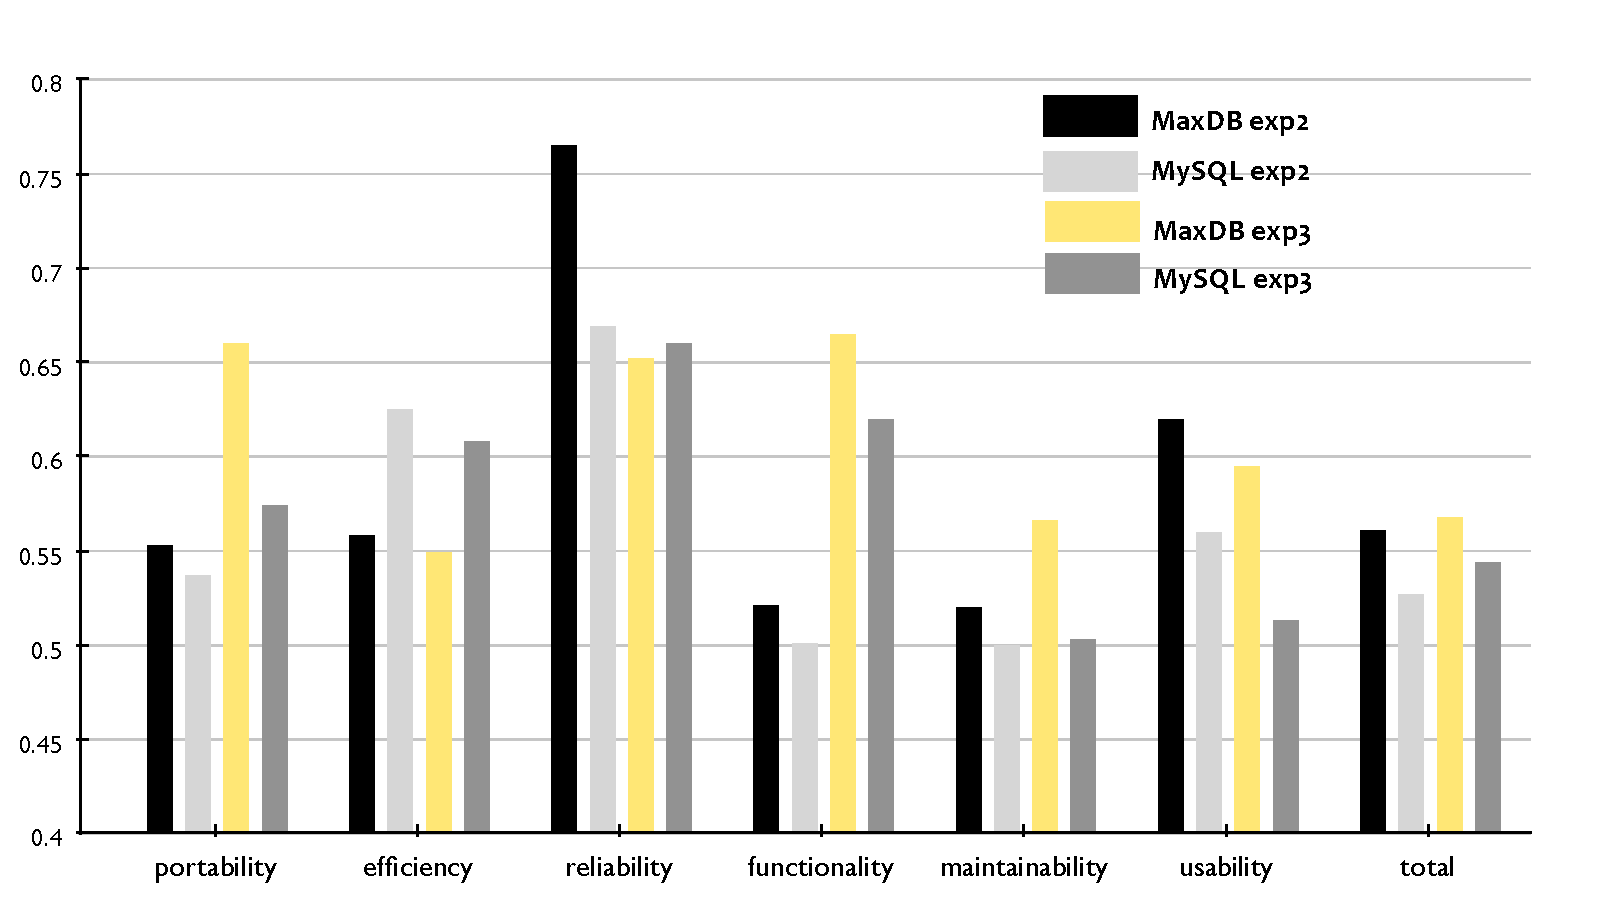
\includegraphics[width=0.45\textwidth]{figures/unsupervised-bar}
% \label{fig:maxdb-unsup-results-roc}
% }
% %\subfloat[F1]{
% %\includegraphics[width=0.45\textwidth]{figures/unsupervised-bar-f1}
% %\label{fig:maxdb-unsup-results-f1}
% %}
% \caption[]{Performance of unsupervised topic labelling for each NFR per word-list. A) ROC values -- dashed line indicates the performance of a random classifier. B) F1 measure. Possible values range from 0--1.
% %\todo[inline]{better discussion}% and graphical legend would be nice}
% }
% \label{fig:maxdb-unsup-results}
% \end{figure}


\begin{figure*}
  \centering
 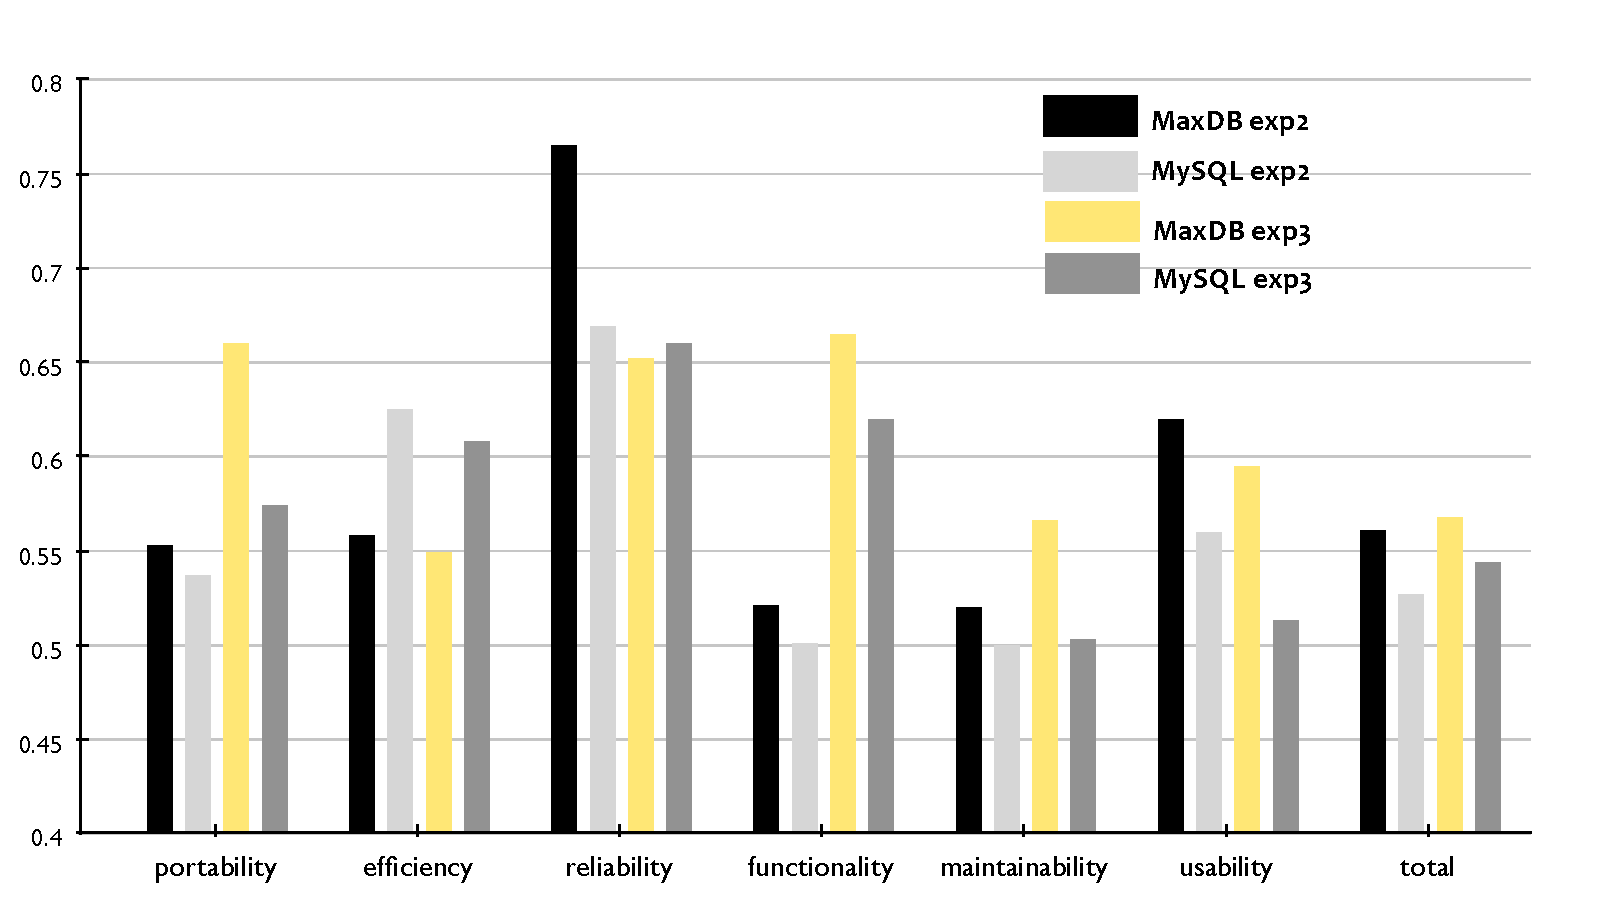
\includegraphics[width=0.8\textwidth]{figures/unsupervised-bar}
 \caption{Performance, ROC values (range: 0-1), of unsupervised topic labelling for
   each NFR and per word-list. Dashed line indicates the performance of a random classifier. This graph shows how well the
   unsupervised topic labelling matched our manual annotations.}

%\todo[inline]{this is too tiny in print}
  \label{fig:maxdb-unsup-results}
\end{figure*}

% \begin{figure}
%   \centering
%  \includegraphics[width=0.45\textwidth]{figures/unsupervised-bar-f1}
%  \caption{Performance, F1 values (range: 0-1), of unsupervised topic labelling for
%    each NFR and per word-list.}
%   \label{fig:maxdb-unsup-results-f1}
% \end{figure}


%\todo[inline]{where is exp1 report?}

%EXP1 could not be evaluated properly!
Because our ground truth annotations were relevant only to ISO9126,
we estimate that \textsf{exp1} had poor
performance via the overlap between ISO-9126 and the Kayed ontology.
For \textsf{exp1} the F-measures for MaxDB were from $0$ to $0.18$ with an average
of $0.03$, and for MySQL were from $0$ to $0.16$ with an average of
$0.05$.
% 0.177215189873 / 6
% .02953586497883333333
% (0.0298507462687 + 0.0661157024793 + 0.0634920634921 + 0 + 0.115384615385) / 6
% .04580718793751666666


% EXP2 source is naming-paper/src/validate/exp2.maxdb.report.txt
% (change as needed). Second column (after the name) is F1.
For \textsf{exp2}, the average F-measure (macro-F1) for MaxDB was $0.24$ with a range $0.091$ to
$0.37$, and $0.16$ for MySQL with a range of $0$ to $0.41$.
MaxDB had an average precision and recall of $0.25$ and $0.22$
while MySQL had $0.41$ and $0.10$ respectively.

% EXP3
For \textsf{exp3}, the average F-measure (macro-F1) for MaxDB was $0.26$ with a range $0.11$ to
$0.47$, and $0.36$ for MySQL with a range of $0.10$ to $0.65$.
MaxDB had an average precision and recall of $0.16$ and $0.67$
while MySQL had $0.3$ and $0.48$ respectively.

Based on these results we find that \emph{reliability} and
\emph{usability} worked well for MaxDB in \textsf{exp2} and better in
\textsf{exp3}. 
\textsf{exp1} performed poorly.
MySQL had reasonable results within \textsf{exp2} for \emph{reliability} and \emph{efficiency}. 
MySQL's results for \emph{efficiency} did not improve in \textsf{exp3} but other qualities such as \emph{functionality} did improve. 
If a \emph{C} grade performance has a ROC value of $0.6$ then most of these tests scored a grade of \emph{C} or less, but our classifier nonetheless performed substantially better than random.


\subsection{Supervised labelling}
\label{sec:suplabelling}
Supervised labelling requires expert analysis of the correct class/label to assign to a topic. In our approach, we use the top-level NFRs in the ISO 9126 standard~\cite{iso9126} for our classes, but other taxonomies are also applicable.%In order to validate how effective these word-bag approaches to topic labelling would be we created a validation data set. 

We used a suite of supervised classifiers, WEKA~\cite{weka09}. 
WEKA includes machine learning tools such as support vector machines and Bayes-nets. 
We also used the multi-labelling add-on for WEKA, Mulan~\cite{mulan}. %\footnote{\url{http://mlkd.csd.auth.gr/multilabel.html}}. 
Traditional classifiers map our topics to a single class, whereas Mulan allows for a mixture of classes per topic, which maps to what we observed while manually labelling topics.

To assess the performance of the supervised learners, we did a 10-fold cross-validation~\cite{Kohavi1995}, a common technique for evaluating machine learners. 
The original data is partitioned randomly into ten sub-samples. Each sample is used to test against a training set composed of the nine other samples.
%One subsample is used as a training set and evaluated on the other nine sub-samples. 
%This is repeated nine more times, with each subsample used once as the training set. 
We have reported these results below.% in Section \ref{sec:suplabelling}.

\subsubsection{Analysis of the supervised labelling}
% \label{sec:suplabelling}
Because our data-set was of word counts we expected Bayesian techniques, often used in spam filtering, to perform well. 
We tried other learners that WEKA~\cite{weka09} provides: rule learners, decision tree learners, vector space learners, and support vector machines.  
Figure \ref{fig:best-learn-per-tag} shows the performance of the best performing learner per label. 
 We considered the best learner for a label to be the learner which
 had the highest ROC value for that label. 
The best learner is important because one uses a single learner per label.
%Figure \ref{fig:best-learn-per-tag} uses the ZeroR learner as a baseline, a common practice in machine learning,
%as ZeroR naively chooses the largest category all of the time. 
%ZeroR occasionally outperforms other learners; for labels which are not as common, this is to be expected because any miscategorization will hurt accuracy. 
%This is why we use ROC values, instead of accuracy, as they can better represent performance on labels which are not applicable to the majority of samples.

Figure \ref{fig:best-learn-per-tag} shows that MaxDB and MySQL have quite different results, as the ROC values for \emph{reliability} and \emph{functionality} seem swapped between projects. 
For both projects Bayesian techniques did the best out of a wide variety of machine learners tested. 
Our best learners, Discriminative Multinomial Naive Bayes, Naive Bayes  and Multinomial Naive Bayes  are all based on Bayes's theorem and all assume, naively, that the features are independent. 
The features we used are word counts per message. 
One beneficial aspect of this result is that it suggests we can have very fast training and classifying  since Naive Bayes can be calculated in $O(N)$ for $N$ features.
%http://nlp.stanford.edu/IR-book/html/htmledition/naive-bayes-text-classification-1.html

% # F measure
% mysql
% > v <- c( 0.64 , 0.23  ,0.41 , 0.77  ,0.62 , 0.21 ) 
% > summary(v)
%    Min. 1st Qu.  Median    Mean 3rd Qu.    Max. 
%   0.210   0.275   0.515   0.480   0.635   0.770 
% maxdb
% > v <- c(0.61, 0.25, 0.59, 0.32, 0.42, 0.17)
% > summary(v)
%    Min. 1st Qu.  Median    Mean 3rd Qu.    Max. 
%  0.1700  0.2675  0.3700  0.3933  0.5475  0.6100 

The range of F-measures for MySQL was $0.21$ to $0.77$ with an average
of $0.48$, while MaxDB had a range of $0.17$ to $0.61$ with an average
of $0.39$.


The less-frequently occurring a label, the harder it is to get accurate
results, due to the high noise level. Nevertheless, these results are
better than our previous word-list results of \textsf{exp2} and
\textsf{exp3}, because the ROC values are sufficiently higher in most
cases (other than MaxDB \emph{reliability} and MySQL \emph{efficiency}). The
limitation of the approach we took here is that we assume labels are
independent; however, labels could be correlated with each other. 
The next section (\ref{sec:multilabel})
addresses the issue of a lack of independence and correlation between labels.
In the next section we will evaluate how well these learners perform
together.
%\todo[inline]{Comment about correlation, we should link to the Mulan section, perfect segway since Mulan relies on correlation.}

\begin{figure}
\centering
% \subfloat[MySQL]{
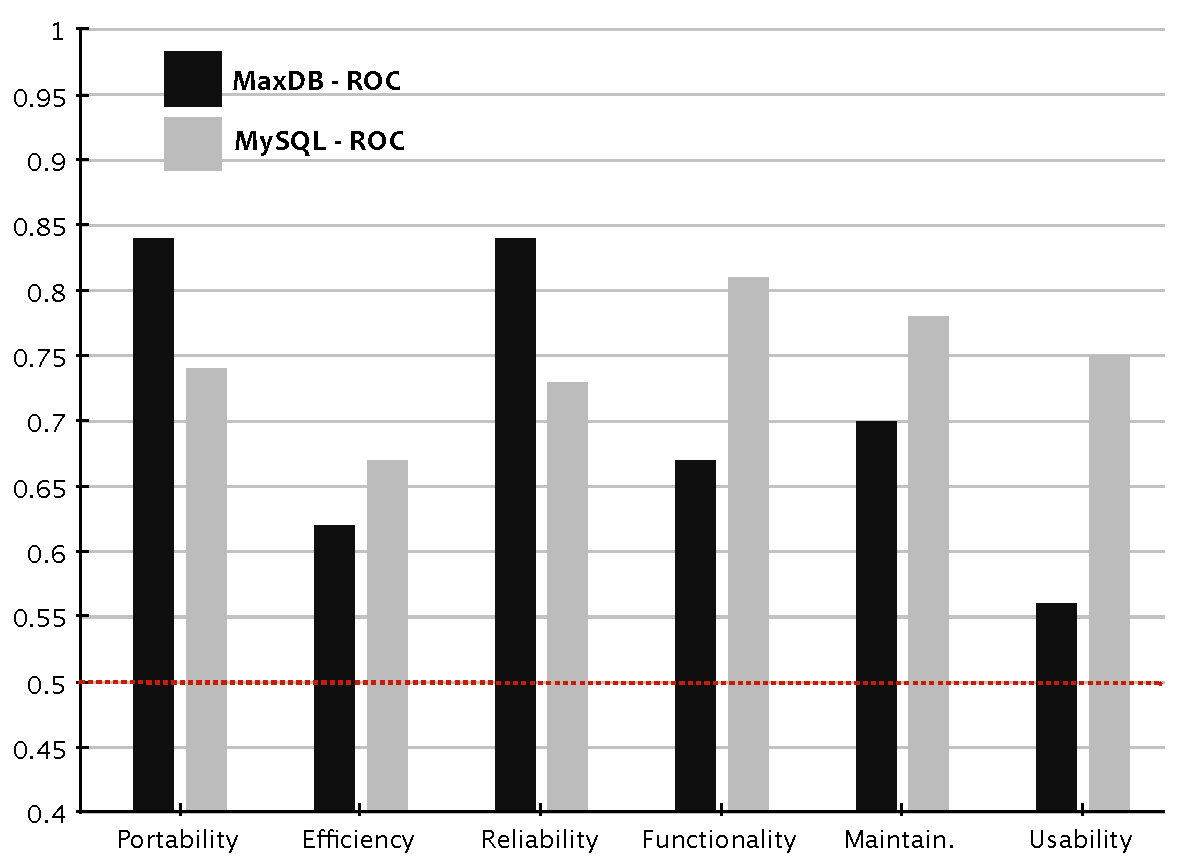
\includegraphics[width=0.4\textwidth]{figures/both-supervised}
% \label{fig:subfig1}
% }
% \subfloat[MaxDB]{
% 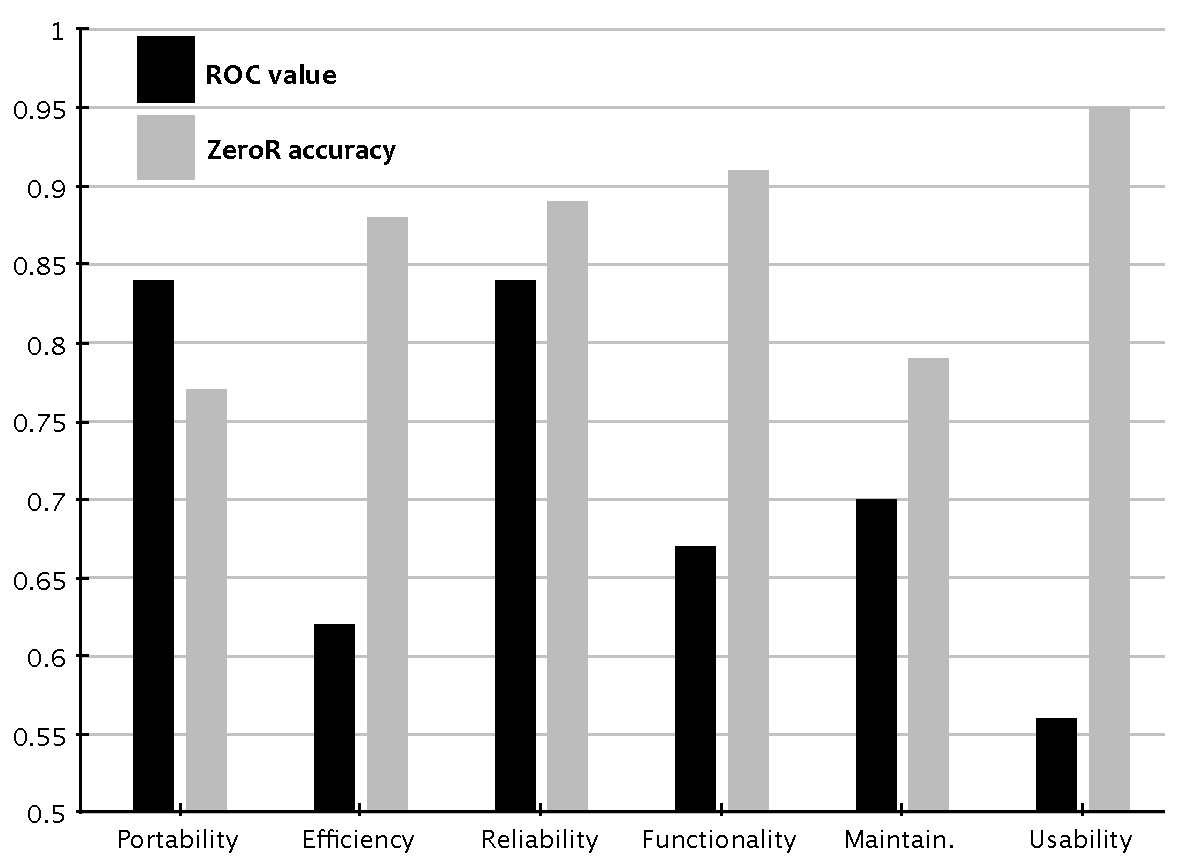
\includegraphics[width=0.4\textwidth]{figures/maxdb-supervised}
% \label{fig:subfig2}
% }
\caption[]{ROC value for the best learner per label for MaxDB and MySQL. Values range from 0--1.  Dashed line indicates the performance of a random classifier.
%\todo[inline]{better discussion}
}
\label{fig:best-learn-per-tag}
\end{figure}

\subsection{Applying multiple labels to topics}
\label{sec:multilabel}

As noted in Section \ref{sec:wordlist}, each topic in our data-set can be composed of zero, one, or more NFRs. 
For example, a commit message might address \textit{reliability} in the context of \textit{efficiency}, or make a \textit{maintainability} improvement in the source code that related to \textit{usability}. 
However, traditional machine learning techniques, such as Naive Bayes, can only map topics to a single class. 
The Mulan~\cite{mulan} library encapsulates several different multi-label machine learners which can label elements with multiple labels.
Mulan also includes methods for determining the performance of such techniques.
% TOO DETAILED The problem framed in the learners above has changed; instead of looking at the precision and recall of applying one label, we rank multiple labels at once. We must check if the full subset of labels was applied, and then how much of that subset was applied.


Two perspectives to evaluate multi-label learners are with micro or macro measurements (used in Figure \ref{fig:mulan}).
Macro measurements are aggregated at a class or label level (per class) while micro measurements are at the element level (per element).
A macro-ROC measurement is the average ROC over the ROC values for all labels, where a micro-ROC is the average ROC over all examples that were classified. 
For MaxDB, the macro-ROC values are undefined because of poor performance of one of the labels.%, see Figure \ref{fig:mulan}.

Figure~\ref{fig:mulan} presents the results of Mulan's best multi-label learners for our data. 
Calibrated Label Ranking (CLR) is a learner that builds two layers, the first layer determines if an entity should be labelled, while the second layer determines what labels should be assigned.
The Hierarchy Of Multi-label classifiERs (HOMER) and Binary Relevance (BR) act as a hierarchy of learners: BR is flat, while HOMER tries to build a deeper hierarchy to build a more accurate learner~\cite{mulan}. 
These classifiers performed better than other multi-label classifiers as they have the best micro and macro ROC scores. 
The multi-label and single-label learners had similar performance: for MySQL, BR and NaiveBayes had similar macro-ROC scores of $0.74$.
% although their results are comparable to the naive Bayesian learners we used in Section \ref{sec:suplabelling}.
% \todo[inline]{discuss this similarity in more detail}

\begin{figure*}[]
\centering
\subfloat[MySQL]{
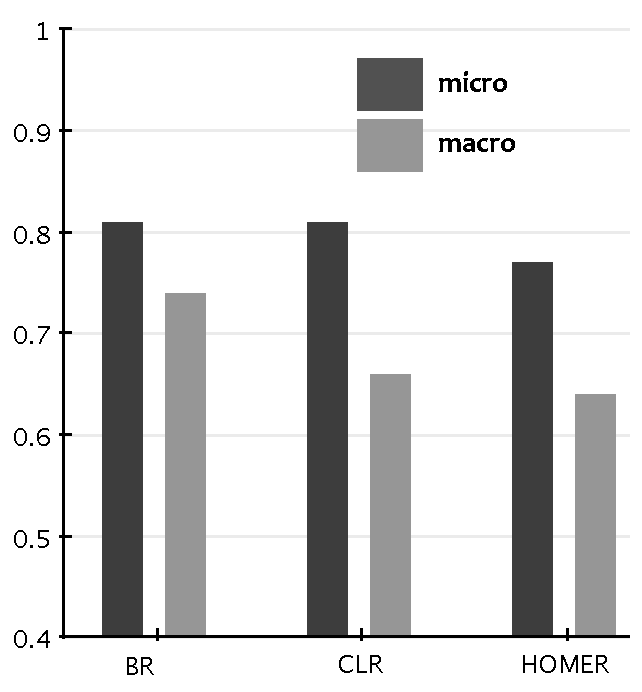
\includegraphics[width=0.3\textwidth]{figures/multi-label-results-mysql}
\label{fig:subfig3}
}
\subfloat[MaxDB]{
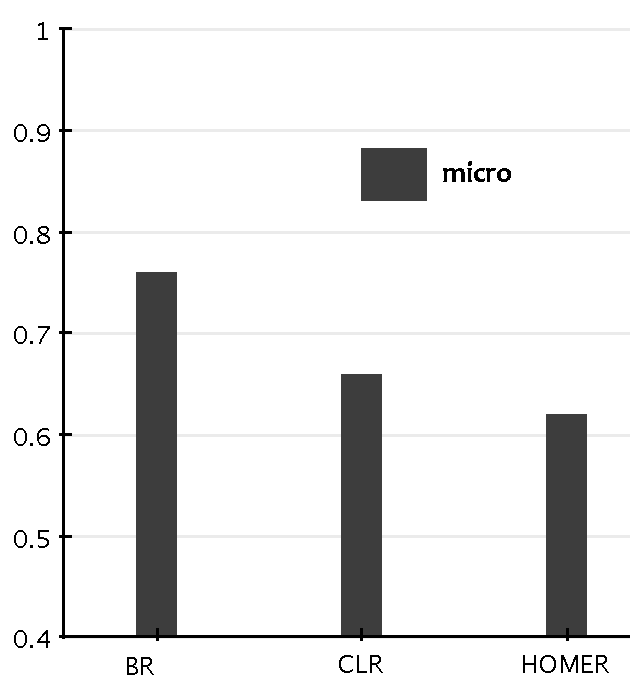
\includegraphics[width=0.3\textwidth]{figures/multi-label-results-maxdb}
\label{fig:subfig4}
}
\caption[]{MySQL and MaxDB macro (grey) and micro (black) ROC results per multi-label learner. Possible values range from 0--1.  Dashed line indicates the performance of a random classifier.
%\todo[inline]{better discussion}% and graphical legend would be nice}
}
\label{fig:mulan}
\end{figure*}

\section{Understanding software maintenance activities} 
\label{sec:analysis}
% \todo[inline]{talk about this topic in one section}
% \todo[inline]{reference project name Nomen more}
%In order to test  our ROC values produced acceptable results, we now turn to
%\emph{applying} those techniques to understand software maintenance
%activities. 
\todo[inline]{more on intro ... why should the reader care about this. It needs to show how the stuff in the intro (applications) is possible}
\todo[inline]{fix section headings}

We evaluated two research questions using the ground truth data that we
annotated by hand:
\begin{enumerate}
\item Do label frequencies change over time? Is a certain quality of more interest at one point in the life-cycle than some other? 
\item  Do the different projects differ in their relative topic interest? Is a particular quality more important to one project than the other projects?  
\end{enumerate}

% There are several possible applications of \textsf{Nomen}'s techniques. 
% For outside users of the software, \textsf{Nomen} can provide insight into that company's development practices. 
% Are they focused on usability, for example?
% Within the organization \textsf{Nomen} acts as a historical sanity check. 
% Confirmation bias is the difference between what people think happened and what actually happened. 
% Some software releases, for instance, are poorly received since they are quite buggy. 
% \textsf{Nomen} would help explain why this was the case, since it can identify NFRs which are dominating developer attention.
%\todo[inline]{does this section use supervised learning, and if so what ones?}

\subsection{Timeline analysis}
Figures \ref{fig:mysql-timeline} and \ref{fig:maxdb-timeline} show the
temporal patterns of label frequencies based on the manually annotated
topics, although this visualization can be generated from the
results of labelled topic extraction.
There are two measures represented. 
One, the relative frequency, shown in the grey boxes, represents the number of labels with that NFR in that period, 
relative to the maximum number of topics assigned to that NFR. 
The second, absolute frequency, compares the number of topics labelled with that NFR per period 
relative to the maximum number of labelled topics overall, for that project. 
The topmost row in each diagram is reserved for historical events of note. 
We refer to these occurrences in the discussion which follows.

%\noindent \textbf{Understanding the figures} -- 
In Figure \ref{fig:mysql-timeline}, we see that the NFRs \emph{functionality}, \emph{portability} and \emph{maintainability} contain more labeled topics, since these NFRs have been more intensely shaded. % boxes. not sure boxes is important..
% I grepped query1.mrs2 http://softwareprocess.es/y/y/maxdb-76.tar.gz
% and                   http://softwareprocess.es/y/maxdb-7500.tar.gz
There are more \textsf{None} labels in MaxDB because a number of topics were to do with code cleanup or automated checking using tools like \texttt{sutcheck}, a tool-specific to the development process at MaxDB. 

%\noindent \textbf{Timeline of key events} -- 
As discussed earlier, the top row in each figure shows key events for each project. 
\textit{Labelled topic extraction} can pick out the underlying NFR activity behind these events. 
For example, both projects show a high number of NFRs recognized at the first period of analysis. 
This is due to our window choice: we deliberately targeted our analysis to when MySQL 3.23 was first announced %Major update \& End-of life
and when MaxDB 7.500 was first announced. For MaxDB, version 7.5.00  was released in December of 2003. 
From analyzing the mailing list for external validation, we know that release 7.5.00.23 saw the development of PHP interfaces, possibly accounting for the simultaneous increase in the \emph{portability} NFR at the same time.
The gap in MaxDB (Figure \ref{fig:maxdb-timeline}) is due to a shift in development focus (from February 2005 to Jun 2005) to MaxDB 7.6, which is released in June 2005.

For MySQL (Figure \ref{fig:mysql-timeline}), we similarly validated our NFR patterns with external mailing list data. 
This release of MySQL was the first to be licenced under the GPL. 
Version 3.23.31 (January, 2001) was the production release (non-beta), and we see a flurry of topics labelled with \emph{functionality} and \emph{maintainability}. 
After this point, this version enters the maintenance phase of its life-cycle. 
In May 2001, there is an increase in the number of topics labelled with \emph{portability}. 
This might be related to release 3.23.38, which focused on Windows compatibility. 
Similarly, in August, 2002, both \emph{functionality} and \emph{portability} are frequent, and mailing list data suggests this is related to the release of version 3.23.52, a general bug fix with a focus on security (a component of the \emph{functionality} NFR in the ISO9126 model). 
After this point, efforts shift to the newer releases (4.0, 4.1, 5.0). 

\begin{figure*}[ht]
\centering
\subfloat[MySQL 3.23]{
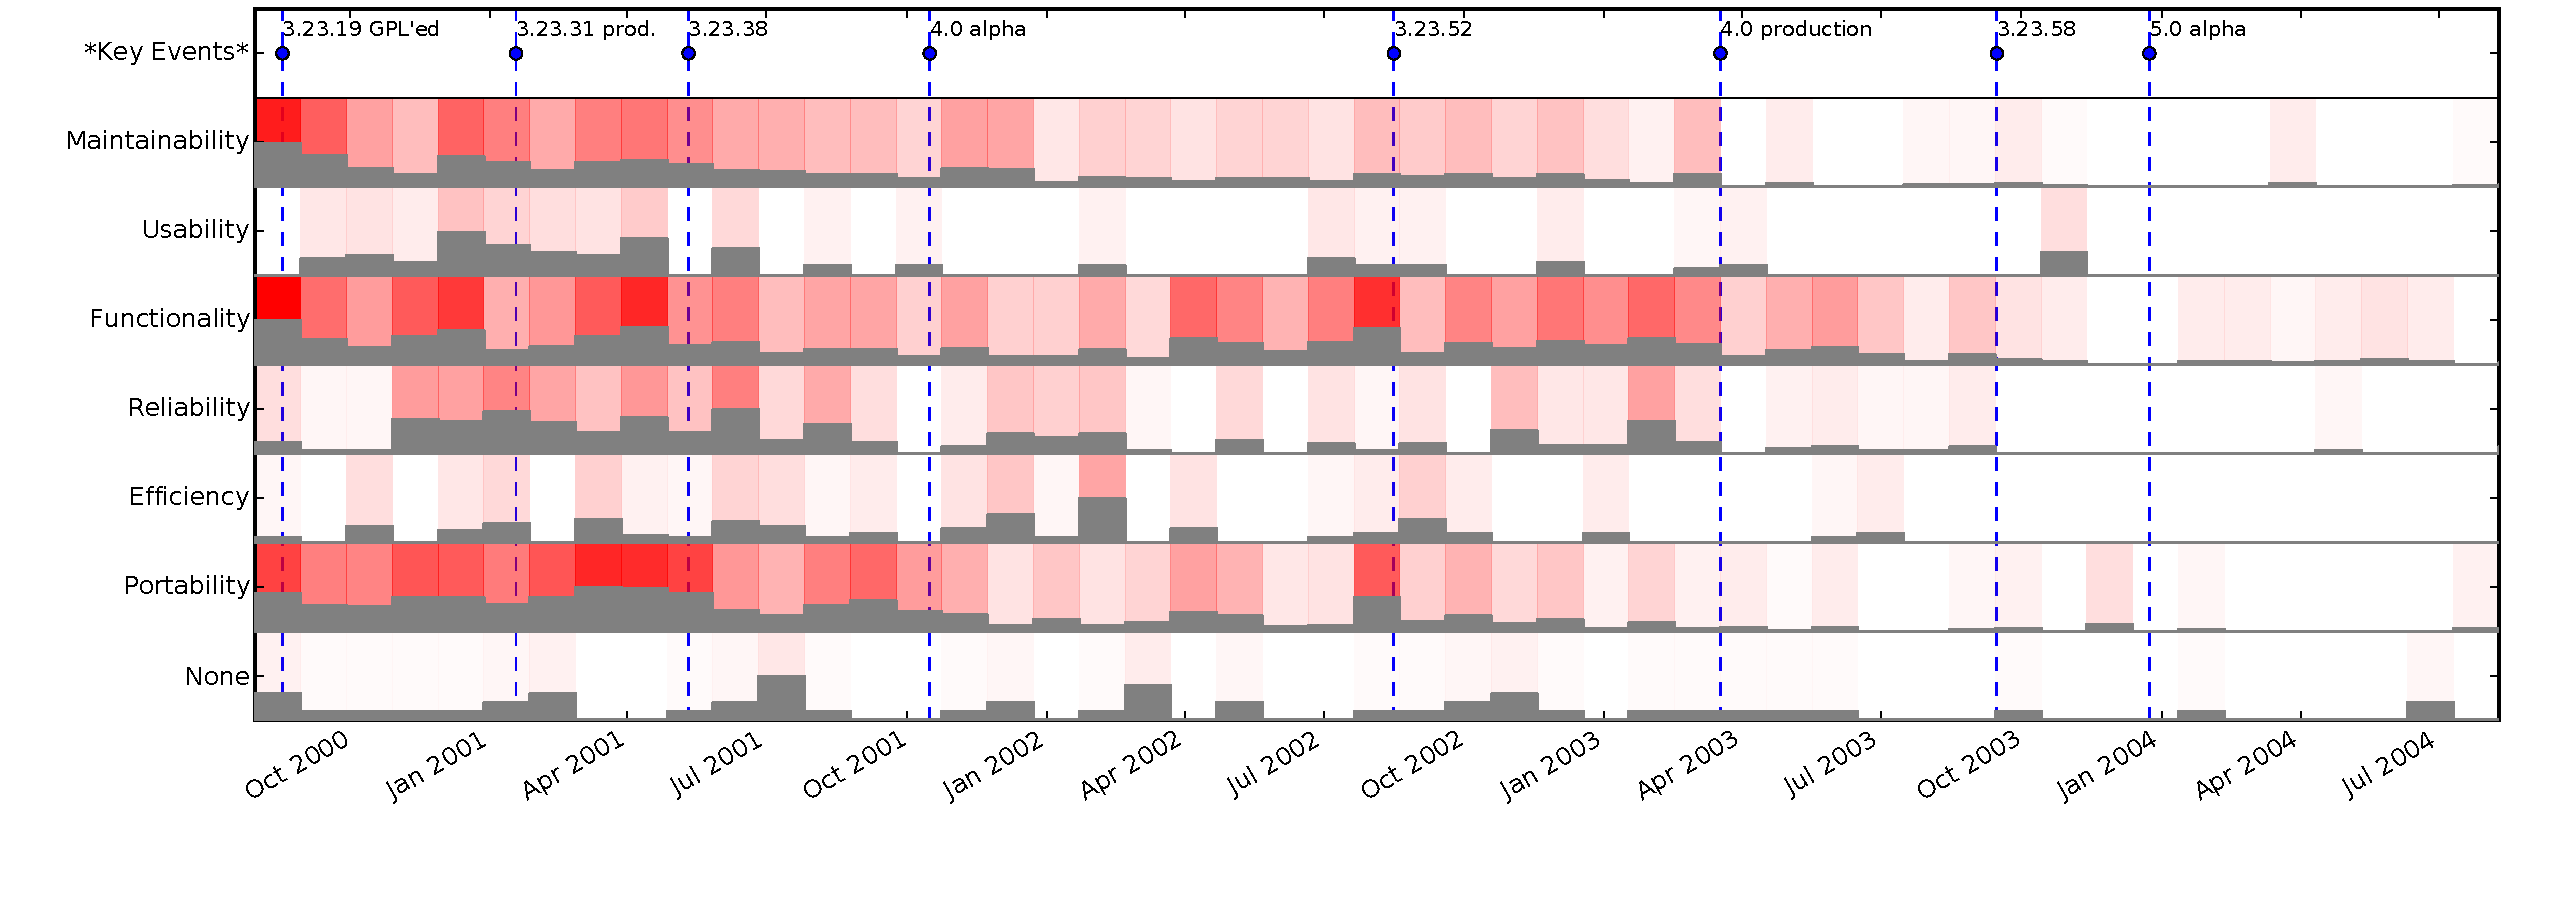
\includegraphics[width=\textwidth]{figures/mysql-timeline}
\label{fig:mysql-timeline}                               
}           
                                             
\subfloat[MaxDB 7.500]{                                 
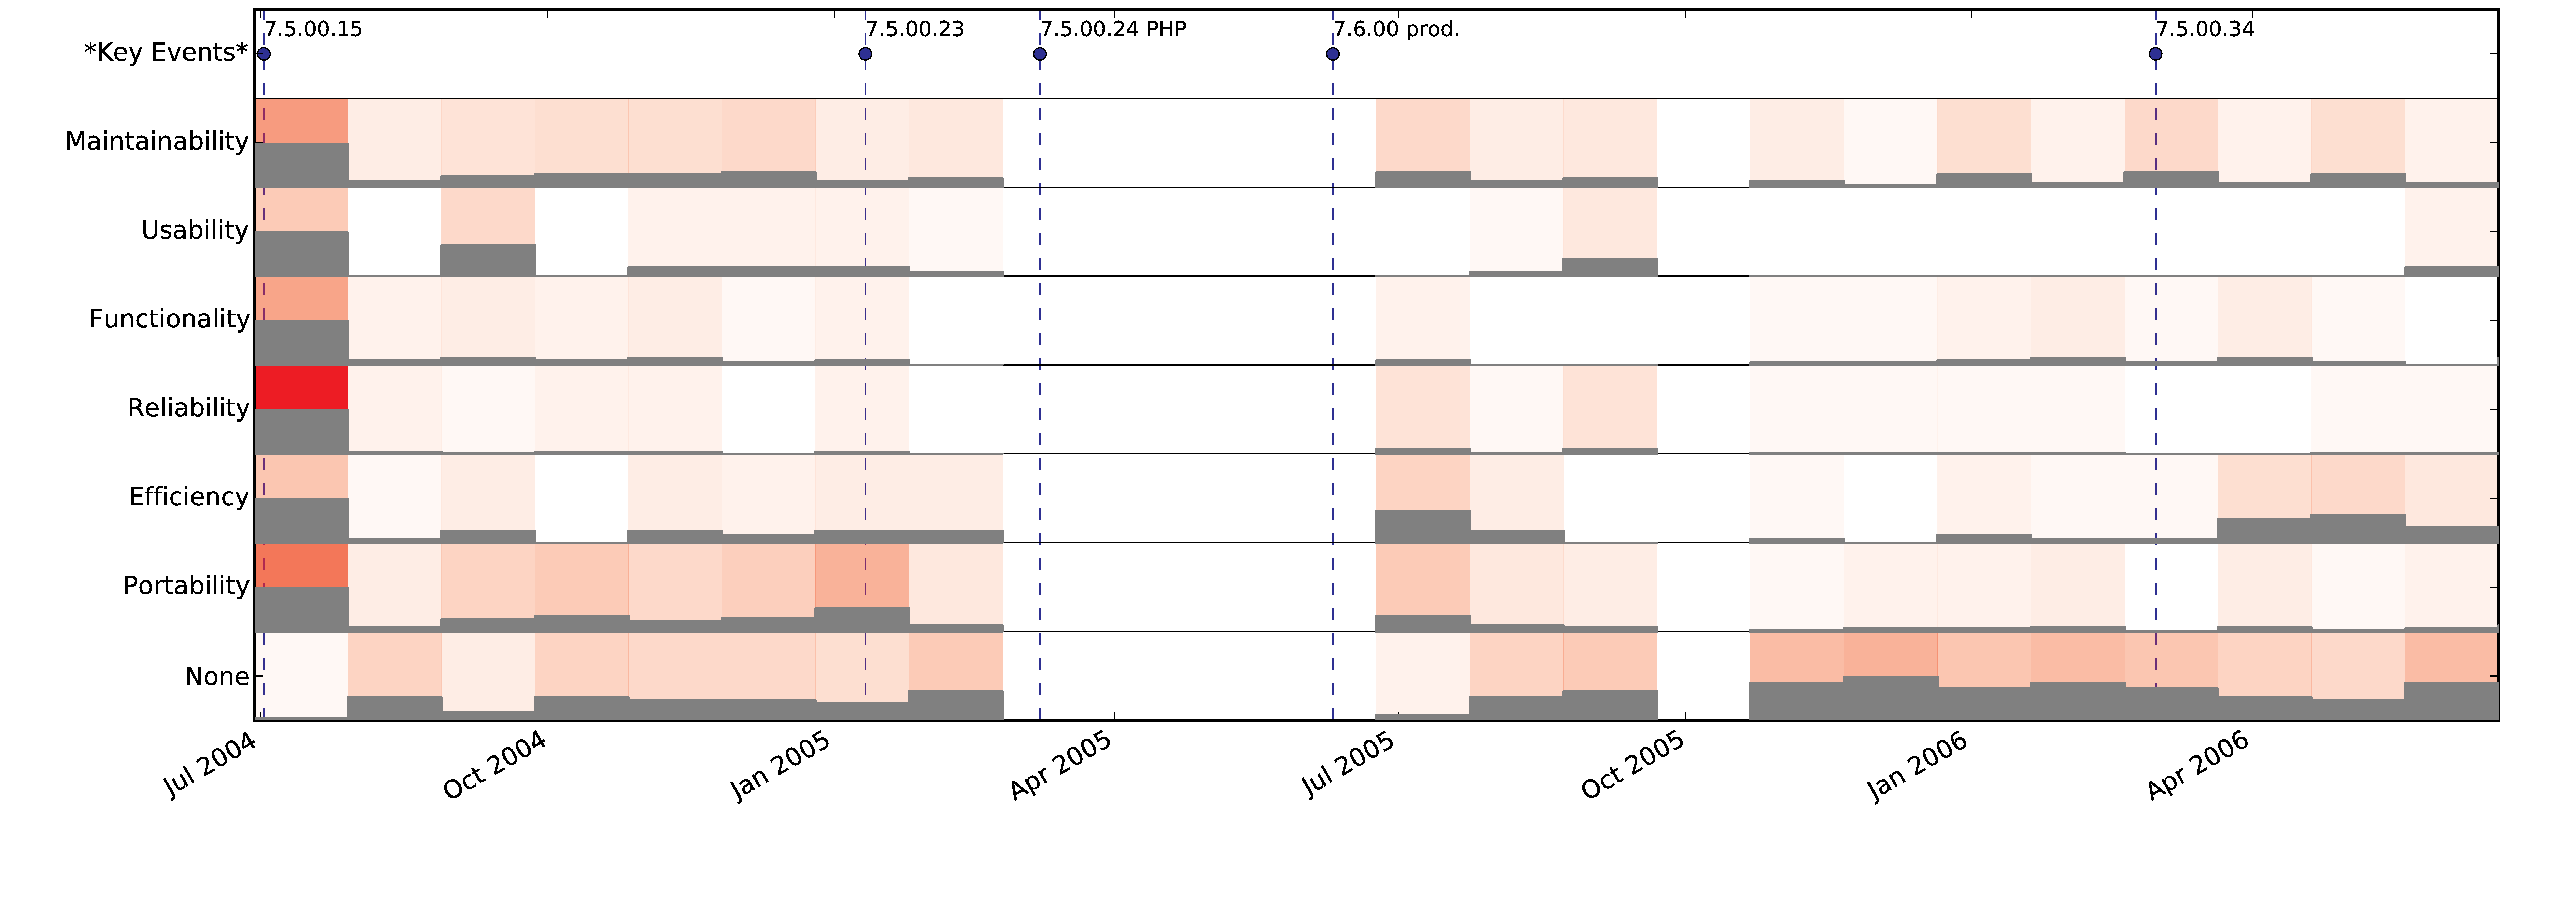
\includegraphics[width=\textwidth]{figures/maxdb-timeline}
\label{fig:maxdb-timeline}
}
	\caption[]{NFR label per period. Each box represents a 30-day period. %Numbers represent number of topics in that period labelled with that NFR. 
	Grid cell intensity (saturation) is mapped to label frequency relative to the largest label value of \emph{all} NFRs. Grey bars indicate label frequency relative to \emph{a particular} NFR. Dashed vertical lines relate a project milestone (*Key Event*) to our topic windows. 
% \todo[inline]{better discussion}
}
\label{fig:timelines}
\end{figure*}

% \subsection{Comparing MaxDB and MySQL}

% \label{sec:comparison}
%\XXX{Not sure there's enough here to do that!}
% We observed that MySQL had more topic subsets than MaxDB. 
% MySQL 3.23 also had more topics and a longer recorded history than MaxDB 7.500. 
% We tagged more MySQL topics with annotations than MaxDB topics, yet both shared similarities. 
% In terms of non-functional requirements both projects had long running trends that focused on \emph{functionality}, \emph{maintainability}, and \emph{portability}, yet MaxDB had more of a focus on \emph{efficiency} and \emph{reliability}. 
% \todo[inline]{expand}
%\todo[inline,color=yellow]{expand on this with dates, and reference to visualizations}

%This analysis allows to address the questions raised in Section \ref{sec:suplabelling}:
This analysis addresses the questions raised in Section \ref{sec:analysis}:

%\textbf{Do label frequencies change over time?} -- 
\subsubsection{Do label frequencies change over time?}
In both projects the frequencies generally decreased with age. 
However, there are variations within our NFR labels. In MySQL, \emph{usability} and \emph{efficiency} do not appear very often in topics. 
A proportionately smaller number of commits addressed these NFRs.
As discussed in the previous section, certain peaks in topic numbers coincide with a particular emphasis from the development team on issues such as new releases or bug fixes.
This suggests that maintenance activity is not necessarily strictly decreasing with time, but rather episodic and responsive to outside stimuli. 
In MaxDB, we can observe that \emph{Maintainability} topics became more prevalent as MaxDB matures. 
This is likely due to our analysis timeframe for MaxDB being shorter than the timeframe for the MySQL product. 



%\textbf{Do the different projects differ in their relative topic
%interest?} -- 

\subsubsection{Do the different projects differ in their relative
  topic interest?}

Yes. MySQL 3.23 had proportionally more
topics labelled \emph{functionality}, while MaxDB had proportionally more
\emph{efficiency} related topics. MaxDB was a very mature release ``donated'' to the open-source community. 
MySQL, on the other hand, was in its relative infancy. 
Security problems were more common (security is a component of `functionality' in the ISO 9126 model). 
In both cases \emph{portability} was a constant maintenance concern and was prevalent throughout the entire lifetime of the projects. 

\todo[inline]{link the actual data, which is interesting, to somethign actionable for a developer or manager}
\section{Discussion}
\label{sec:limit}

%XXX can just remove this
%\subsection{Effectiveness}
\subsection{Annotation observations}
We found many topics that were not non-functional requirements (NFRs) but were often related to them. 
For instance, concurrency was mentioned often in the commit logs and
was related to \emph{correctness} and \emph{reliability}, possibly because concurrent code is prone to bugs such as race conditions. %are 
% often  was troublesome. 
\emph{Configuration management} and \emph{source control} related changes appeared often; % and sometimes there were topics dedicated to configuration management. 
these kinds of changes are slightly related to \emph{maintainability}. 
A non-functional change that was not quality-related was licensing and copyright; many changes were simply to do with updating copyrights or ensuring copyright or license headers were applied to files. In these cases we assigned the \emph{None} class.

We noticed that occasionally the names of modules would conflict with words related to other non-functional requirements. 
For instance, optimizers are very common modules in database systems: both MySQL and MaxDB have optimizer modules. 
In MySQL the optimizer is mentioned but often the change addresses  correctness or another quality. 
Despite this difference, the name of the module could fool our learners into believing the change was always about \emph{efficiency}. 
In these cases the advantages of tailoring topic names to specific project terminologies are more clear. 
Project specific word-lists would avoid automated mistakes due to the names of entities and modules of a software project.

\subsection{Summary of techniques}
While an unsupervised technique such as LDA is appealing in its lack of human intervention, and thus lower effort, 
supervised learners have the advantage of domain knowledge, which typically means improved results. 
% NEIL - we got criticized for making it sound like this is the obvious thing to do... and then why do you need a learner?
%Our manual annotations were fairly quick to do, taking only a few minutes per 30 day period. 
Creating annotated topics (i.e., manual labels) for training is painstaking, but with a suitably representative set of topics, the effort is acceptable. To annotate \emph{all} topics took us approximately 20 hours per project, but we estimate only 10\% of the topics need annotation to produce useful results.

Very rarely did \textsf{exp2} and \textsf{exp3} (unsupervised word matching) ever perform as well as the supervised machine learners. 
For MaxDB, \textit{reliability} was slightly better detected using the static word list of \textsf{exp2}. 
In general, the machine learners and \textsf{exp3} did better than \textsf{exp2} for both MaxDB and MySQL. 
For both MySQL and MaxDB \textit{usability} was better served by \textsf{exp2}. 
\textit{Usability} was a very infrequent label, however, which made it difficult to detect in any case.

We found that the multi-label learners of BR, CLR and HOMER did not do as well for Macro-ROC as NaiveBayes and other naive Bayes derived learners. 
This suggests that by combining together multiple NaiveBayes learners we could probably label sets of topics effectively, but it would require a separate NaiveBayes learner per label.

%{Discuss how these are CHEAP techniques and although somewhat %inaccurate they don't require a tonne of work}
The unsupervised labelling had difficulty distinguishing between common labels and infrequent labels. 
The learners would occasionally mislabel a topic deserving of an infrequent label with a more common label.
The word-lists for \emph{correctness} tended to be too lengthy, non-specific and broad, especially if WordNet words were used, since the NFRs are typically loosely defined concepts in common parlance.

With ROC values ranging from $0.6$ to $0.8$ we can see there is promise in these methods.
\textsf{exp2} and \textsf{exp3} both indicate that static information can be used to help label topics without any training whatsoever. 
MySQL and MaxDB's machine learners made some decisions based off a few shared words: \textsf{bug, code, compiler, database, HP UX, delete, memory, missing, problems, removed, add, added, changed, problem, and test}. 
Adding these words to the word-lists of \textsf{exp2} and \textsf{exp3} could improve performance while ensuring they were only domain specific.

If the techniques used in \textsf{exp2} and \textsf{exp3} were combined with the supervised techniques, we could reduce the training effort by boosting training sets with topics classified with the unsupervised techniques.
Both Naive Bayesian learners and the word-list approaches were computationally efficient.  
%These results are promising, because the accuracy of the techniques is good enough to be useful, while the run-time performance is still cheap enough to execute to be feasible as an automated or semi-automated method of labelling topics by their software qualities.
These results are promising because they indicate that these techniques are accurate enough to be useful while still maintaining acceptable run-time performance.

\subsection{Threats to validity}
% can always be cut down
%Our work faced multiple threats to validity and we attempted to address many of them.
\emph{Construct validity} -- we used only commit messages rather than mail or bug tracker messages. Since we required a seamless record, it was not possible to obtain other data sources. Possibly they would have influenced our results, but there would be a degree of correlation between the corpora.
%Conversely, construct validity was addressed in our validation as we used the files, topics and revisions to annotate the commit messages. 
%We used mailing-lists to verify the purpose behind some events.
Our taxonomy for software NFRs is subject to dispute, but seems generally accepted. Finally, there are exogenous sources, such as in-person discussions, which we did not access, an omission as noted in \cite{aranda09icse}. %We did not show these results to the stakeholders.

\emph{Internal validity} -- %includes inter-rater reliability and our lack of rival explanation building. 
We improved internal validity by trying to correlate and explain the behaviours observed in the analysis with the historical records of the projects.
We did not attempt to match our results to any particular model or theory, as such theories are sparse in 

\emph{External validity} -- %was addressed by our use of two case studies, but there are still issues. 
Our data originated from OSS database projects and thus might not be applicable to commercially developed software. 
Furthermore, our analysis techniques rely on a project's use of meaningful commit messages. The OSS projects investigated were database systems, thus 
our results might not generalize to other domains. %We only studied database systems.
% \todo[inline]{If we compare with the same domain we don't get to say it generalizes a lot?}

% in Case Study Research: Design Case Studies
\emph{Reliability} -- each annotator followed the same protocol and used the same annotations. 
However, only two annotators were used; their annotations could be biased as we did not analyze for inter-rater reliability.

\subsection{Future work}
There are several avenues of further investigation.  
More external validation would be useful. 
Although we validated our comparisons using a mailing list for each project, interviews with developers would provide more detail. 
We also think multi-label learning techniques, although in their infancy, are crucial in understanding cross-cutting concerns such as NFRs. 
We want to leverage different kinds of artifacts to discover threads of NFR-related discussions that occur between multiple kinds of artifacts.
Finally, we would like to extend this analysis to other domains, to see what patterns might occur in, for example, a consumer-facing software product.

\section{Conclusions}
This paper presented a cross-project data mining technique,
\emph{labelled topic extraction}. The technique leveraged a
non-functional requirements (NFRs) taxonomy to mine and label latent
software development topics. Previous topic analysis research produced
topics that needed to be manually labelled, but topics without labels
are difficult to interpret, and manually labelling them is
costly. Furthermore, previous work was project specific and incomparable. 
To improve this, we leveraged software engineering standards, specifically the ISO quality taxonomy, to produce a method of supervised and unsupervised topic labelling.
Since the word-list technique is not project specific, it can be used to compare multiple projects.%topics and artifacts from project histories.
% Our contributions include:
% \begin{itemize}
% \item We provided an unsupervised method of topic labelling (word-lists);
% %\item Our unsupervised method can be applied to projects without training;
% \item We demonstrated a supervised method of labelling topics by a single NFRs (machine learning);
% \item We demonstrated a supervised method of labelling topics by multiple NFRs (multi-label machine learning);
% \item We provided a method of cross-project analysis via topic labelling;
% \item We demonstrated a method of visualizing these topics across time, which we used to analyze maintenance activities.
% \end{itemize}

We validated our topic labelling techniques using multiple experiments. 
We first conducted unsupervised labelling using word-lists. 
Our next approach was supervised, using single-label and multi-label learners. 
Both kinds of learners performed well with average
%area under the 
ROC values between $0.6$ and $0.8$. These results, along with the efficient performance of our learners, demonstrates that labelled topic extraction is a promising approach for understanding 

These labelling techniques allowed us to investigate the occurrence of non-functional requirements in our projects. 
%Although it may seem like common knowledge that maintenance is a concern as a project matures, our technique was able to show this independently.
We showed that NFRs are often trending topics in commit comments
%, and that NFRs are quite common as developer topics.
%; and that there are efficient methods of automating topic labelling.

%%%HMMM


% We demonstrated multiple supervised and unsupervised methods of topic labelling, including multi-label learners.
% We provided a case study and visualization of NFR related topics in MaxDB 7.500 and MySQL 3.23. 
% During the case study we manually labelled hundreds of topics by hand and then used these annotations to validate the positive performance of topic labelling techniques.
% The implication of our paper is that topics with labels are more useful for analyzing software development activities than are unlabelled topics. To furnish stakeholders with labelled topics, our technique provides many methods of automatic topic labelling.

\appendix

Our data and scripts are available at:

 \url{http://softwareprocess.es/nomen/}

\bibliographystyle{abbrv}
%\bibliographystyle{IEEEtran}
\bibliography{icpc}

\end{document}

%%% Unused stuff from conclusions
%\todo[inline]{Need to juxtapose our work against previous work -- contribution}
%\todo[inline]{tighten... typically conclusions are much shorter.}

% What did we do
% What did we show
% What did we do that was new?

% para 1 we did this, we were successful
% We found NFRs
% Our manual inspection and annotation of the topics extracted from MySQL and MaxDB revealed that many of the extracted topics dealt with NFRs, and these topics were spread across the entire history of a project. 
% Try to provide an example of NFRs but little context
%too specific in this sectionIn the cases of MaxDB and MySQL, portability was a constant maintenance concern and was prevalent throughout the entire lifetime of the projects.


%XXXXXXXXXXXXXXXX I think we need to suggest a couple of uses.


% para 4 summarize and hammer contribution
% NE not a fan of this phrasing -> % In conclusion,

%We leveraged word-bags, machine learning classifiers and multi-label machine learning classifiers.  
%We evaluated these techniques using multiple experiments against two open source database systems and visualized the results.
%We found that our topic labelling techniques were effective.

% para 2 we did this to validate and show we did it
% Experiment description -- origin of wordbags
% NEIL - shortening this 

 % Talk to people
% We want to investigate developer attitudes related to these labels: i.e., when we label a topic, was the developer expressing positive or negative qualities about that label?  
% It is difficult to map abstract qualities to particular messages. % what?
%  % This is disjointed and needs more context
% On question we seek to answer is if a ``quality'' discussion about more than just corrective maintenance? %In this study we take the position that any type of maintenance has to do with software quality.
% Using unsupervised word-list analysis we set up two NFR topic labelling experiments: 
% our \textsf{exp2} experiment used small but accurate word-lists, while \textsf{exp3} used large general word-lists derived from WordNet.
% The performance of these techniques differed per NFR but both \textsf{exp2} and \textsf{exp3} had similar performance.
%Our \textsf{exp2} experiment used small accurate word bags to label topics but performed just as well as \textsf{exp3}, which used many more general terms from WordNet.
% we could can improve auto labelling with ML
% Our third experiment showed that with some supervision, and by using efficient machine learners based on Naive Bayesian classifiers, we could improve the accuracy of automatic topic labelling even further.
% Our fourth experiment evaluated the effectiveness of multi-label learners, such as HOMER. 

% \begin{comment}
%  shared-report.sh ; cat output/shared-j48-words 
% 
%       2 bug
%       2 code
%       2 compiler
%       2 database
%       2 Delete_
%       2 HP_UX
%       2 memory
%       2 missing
%       2 monty_mysql_com
%       2 monty_mysql_fi
%       2 problems
%       2 Removed
%       2 work__home_bk_mysql
%       4 4_0
%       4 Add
%       4 added
%       4 Changed
%       4 problem
%       6 Added
%       6 test
% 
% \end{comment}



% \begin{comment}
% A quick mind dump before I forget:
% * portability was very popular
% * there were many instances of concurrency
% * There were often topics of crap commits with no comment
% * might need more than the top words to compare
% * Things like tests were noticable more by file type
% * Configuration management is not part of the software quality ontology?
% * I didn't tag none I tagged unknown, so that's some inconsistency between us
% * There were a lot of copyright changes in mysql
% * mysql had optimizer module which did not mean optimization
% * I tried to assign reliability/bug for reliability bugs
%   and Functionality/Correctness for fixes
% * some security changes came later
% * Mysql 3.23 transitioned from a project being developed to
%   a project being maintained, more frequent back-port bug-fixes
% \end{comment}
% % a rough sketch 
% The size of these artifacts is cumbersome for a developer or stakeholder to comprehend, thus they often have to be ``chunked'', grouped, modularized, organized and finally labelled.
% Even more difficult is to pull together tangible trails or interests that pervade these artifacts.
% These interests or topics are only really visible by analyzing multiple artifacts.
% Other researchers have focused on extracting these topics from development artifacts, but often their approach leaves the organization or the labelling step to the user.
% What we propose is to 
% In this paper, we seek to automatically extract these interests, or topics that link artifacts such as source control commits and label them.

% % Read for SE Data Mining
% % Read for Topic Naming
% % Read for previous research DID NOT
% % thoughts, what does this do what are we introducing
% % these abstractions ... how to link them

% The act of developing software generates many artifacts, including source code, bug reports, commit messages, and test cases. 
% It does not take long for a software project to grow to a point where keeping track of these artifacts exceeds easy comprehension. 
% For these projects, developers interact with abstractions of these artifacts, rather than the artifact itself. Such abstractions include project dashboards~\cite{kersten2005mylar}, tags~\cite{treude2010}, and complexity metrics \cite{mccabe1976complexity}. 


% Developers do more than merely observe these abstractions, however. They must also use them to assess progress and work with colleagues. To have meaningful discussions about how software development is progressing, we must be able to devise appropriate labels for our development artifacts. Such labels can be used to compare progress or understand how well a project is meeting requirements. These labels then become the topics for development conversations (such as the stream of commentary on a bug report). One way to identify topics is to use the artifacts themselves to derive them. 
% \todo[inline]{it should be labels for topics not artifacts, I think the artifact part is almost secondary and the topic stuff is really what is up. Topics are used below and it isn't even clear what they are or what we're talking aout. Naming is important but lets tell the reader what is being named first.}

 %\todo[inline]{Future work is disjointed the question should be more clear}


% Be careful how you merge!

% We demonstrated that static but domain-specific knowledge can improve unsupervised labelling of extracted topics. Our \textsf{exp2} experiment used small accurate word bags to label topics but performed just as well as \textsf{exp3}, which used many more general terms from WordNet. We then showed that with some supervision, and by using efficient machine learners based on Naive Bayesian classifiers, we could improve the accuracy of automatic labelling topics even further.

% Our manual inspection and annotation of the topics extracted from MySQL and MaxDB revealed that many of the extracted topics dealt with non-functional requirements, and these topics were spread across the entire history of a project. In the cases of MaxDB and MySQL, portability was a constant maintenance concern and was prevalent throughout the entire lifetime of the projects.

% We showed that non-functional requirements are often trending topics, that non-functional requirements are quite common in developer topics, and that there are efficient methods of semi-automating and automating topic labelling.

% There are several avenues of further investigation.  We want to investigate developer attitudes related to these labels: i.e., when we label a topic, was the developer expressing positive or negative qualities about that label?  It is difficult to map abstract qualities to particular messages. Is a ``quality'' discussion about more than just corrective maintenance? %In th
%is study we take the position that any type of maintenance has to do with software quality.

%XXX can save space here!
%\section{Appendix}
